% HMBC paper presentation — Team 17, Research in Information Security
% Compile with XeLaTeX or LuaLaTeX (Metropolis uses the Fira Sans fonts), e.g.:
%   tectonic -X compile hmbc-presentation.tex      (or: latexmk -xelatex hmbc-presentation.tex)
% Figures 1 and 11 are taken from the paper (CC BY 4.0); the other diagrams are redrawn from it.
% Slides 9-14 cover JANUS (Appl. Sci. 2023), our RQs and our stack; slides 15-24 cover Phase E (RQ1) and slide 25 what comes next
% (status as of 2026-10-12: gate E PASS, board at F0).
\documentclass[aspectratio=169,10pt]{beamer}
\usetheme[progressbar=frametitle,numbering=fraction,block=fill]{metropolis}
% Fira Sans Light is Metropolis' regular weight; use SemiBold so bold text stands out.
\setsansfont[BoldFont={Fira Sans SemiBold},ItalicFont={Fira Sans Light Italic},BoldItalicFont={Fira Sans SemiBold Italic}]{Fira Sans Light}

\usepackage{tikz}
\usetikzlibrary{arrows.meta,positioning,calc,fit,shapes.symbols}
\usepackage{pgfplots}
\pgfplotsset{compat=1.18}
\usepackage{booktabs}
\usepackage{pifont}
\usepackage{colortbl}
\newcolumntype{L}[1]{>{\raggedright\arraybackslash}p{#1}}

% Colours: proxy chain purple and hospital chain green as in the paper's Fig. 1; Metropolis orange as accent.
\definecolor{pbc}{HTML}{7030A0}
\definecolor{dbc}{HTML}{548235}
\definecolor{datagray}{HTML}{6B6B6B}
\definecolor{accent}{HTML}{EB811B}
\definecolor{okgreen}{HTML}{2E7D32}
\definecolor{badred}{HTML}{C62828}
\newcommand{\cmark}{\textcolor{okgreen}{\ding{51}}}
\newcommand{\xmark}{\textcolor{badred!80}{\ding{55}}}
\newcommand{\pmark}{\textcolor{okgreen!80}{(\ding{51})}}
\newcommand{\src}[1]{{\scriptsize\color{datagray}#1}}
% Project status shown on slides 11 and 16; updated with each hourly refresh from the agent branches.
\newcommand{\statusstamp}{12 Oct 2026, gate E PASS}
% Result classes of the RQ1 catalog (Phase E slides): a 4-slot categorical set; gray = undecided (BLOCKED).
\definecolor{clsup}{HTML}{3A6FB0}
\definecolor{clgap}{HTML}{EB811B}
\definecolor{clrep}{HTML}{2E7D32}
\definecolor{clblk}{HTML}{9A9A9A}
\newcommand{\cls}[2]{\tikz[baseline=(n.base)]\node[draw=#1, fill=#1!14, rounded corners=1.5pt, inner sep=1.2pt, font=\tiny\bfseries] (n) {#2};}
\newcommand{\cSup}{\cls{clsup}{SUPPORTED}}
\newcommand{\cGap}{\cls{clgap}{SPEC\_GAP}}
\newcommand{\cRep}{\cls{clrep}{REPAIR\_SUPPORTED}}
\newcommand{\cBlk}{\cls{clblk}{BLOCKED}}
\newcommand{\code}[1]{{\ttfamily\scriptsize #1}}
\newcommand{\gapn}[1]{\tikz[baseline=(g.base)]\node[circle, fill=accent, text=white, font=\scriptsize\bfseries, inner sep=1.2pt, minimum size=0.42cm] (g) {#1};}
% \wcells{group x}{first index}{y}{count}{colour}: one square per catalog row (slide "Gate E").
\newcommand{\wcells}[5]{\foreach \k in {1,...,#4}{\fill[#5, rounded corners=0.5pt] ({#1+(#2+\k-1)*0.26},#3) rectangle ++(0.22,0.22);}}
\newcommand{\seqmsg}[5]{\draw[msg, #5] (#1,#3) -- node[lbl, above] {#4} (#2,#3);}

\tikzset{
  >={Stealth[length=2mm]},
  box/.style={draw, rounded corners=2pt, align=center, inner sep=3pt, font=\scriptsize, execute at begin node={\hyphenpenalty=10000}},
  lane/.style={box, minimum width=1.45cm, minimum height=0.5cm, font=\scriptsize\bfseries},
  msg/.style={->, thick},
  lbl/.style={font=\scriptsize, fill=white, inner sep=1pt},
  stat/.style={draw=#1, fill=#1!7, rounded corners=3pt, text width=3.05cm, minimum height=1.6cm, align=center, inner sep=4pt, font=\scriptsize},
  prof/.style={draw=#1, fill=#1!9, rounded corners=2pt, text width=4.95cm, align=left, inner sep=3pt, font=\scriptsize},
  pcard/.style={draw=#1, rounded corners=3pt, align=left, inner sep=5pt, font=\scriptsize, anchor=north},
  phead/.style={fill=#1, rounded corners=3pt, inner sep=4pt, text=white, anchor=south},
  dv/.style={draw=#1, fill=#1!10, rounded corners=1.5pt, minimum width=0.98cm, minimum height=0.62cm, align=center, inner sep=1pt, font=\tiny},
  tile/.style={draw=#1, fill=#1!10, rounded corners=3pt, text width=2.3cm, minimum height=1.7cm, align=center, inner sep=3pt},
}

\title{A Hierarchical Multi Blockchain for Fine Grained Access to Medical Data}
\subtitle{Malamas, Kotzanikolaou, Dasaklis \& Burmester \,·\, IEEE Access, vol.~8, 2020}
\author{Saiyam \,·\, Hemang \,·\, Eashaan}
\institute{Research in Information Security \,·\, Mid presentation}
\date{}
\titlegraphic{%
  \begin{tikzpicture}[remember picture, overlay]
    \node[anchor=south east, inner sep=0pt] at ([xshift=-0.6cm, yshift=0.55cm]current page.south east)
      {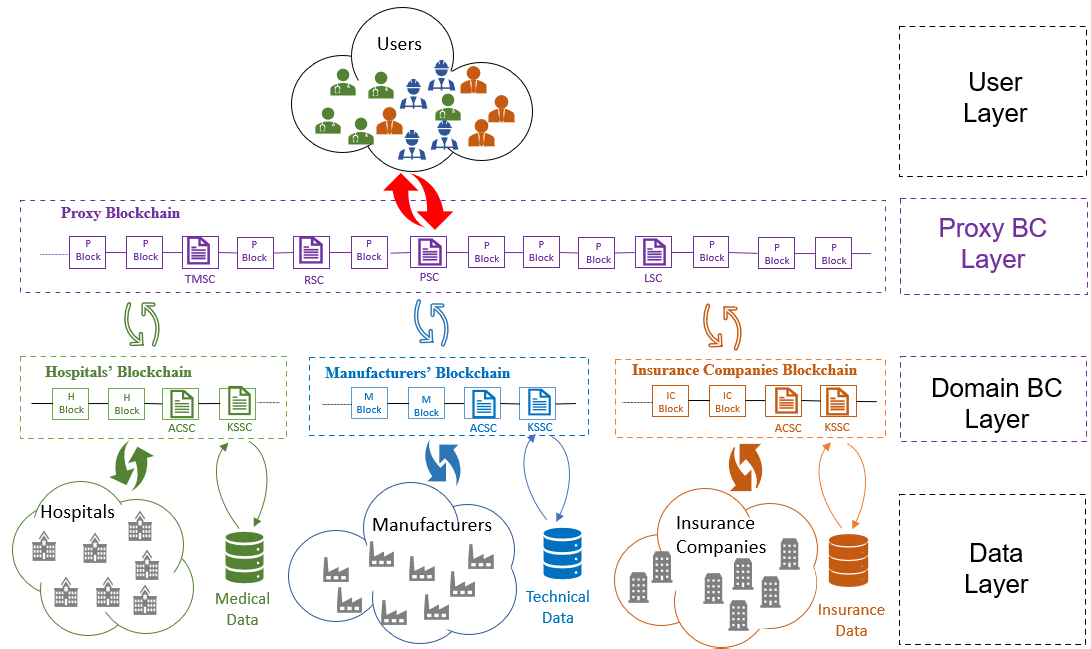
\includegraphics[height=2.9cm]{figures/fig1-architecture.png}};
  \end{tikzpicture}}
\hypersetup{pdftitle={HMBC: A Hierarchical Multi Blockchain for Fine Grained Access to Medical Data (Team 17)}}

\begin{document}

% ---------------------------------------------------------------- 1. Title
\maketitle

% ---------------------------------------------------------------- 2. Context
\begin{frame}{Why was this needed?}
\begin{columns}[c,onlytextwidth]
\column{0.42\textwidth}
\centering
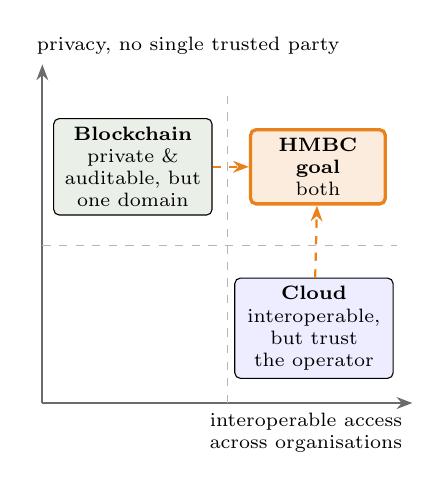
\begin{tikzpicture}
  \draw[->, thick, datagray] (0,0) -- (4.7,0) node[below left, font=\scriptsize, text=black, align=right] {interoperable access\\across organisations};
  \draw[->, thick, datagray] (0,0) -- (0,4.3) node[above right, font=\scriptsize, text=black, align=left, xshift=-0.2cm] {privacy, no single trusted party};
  \draw[dashed, datagray!50] (2.35,0) -- (2.35,4.0);
  \draw[dashed, datagray!50] (0,2.0) -- (4.5,2.0);
  \node[box, fill=blue!7, text width=1.8cm] (cloud) at (3.45,0.95) {\textbf{Cloud}\\interoperable, but trust the operator};
  \node[box, fill=dbc!12, text width=1.8cm] (bc) at (1.15,3.0) {\textbf{Blockchain}\\private \& auditable, but one domain};
  \node[box, draw=accent, very thick, fill=accent!15, text width=1.5cm] (hmbc) at (3.5,3.0) {\textbf{HMBC goal}\\both};
  \draw[->, accent, thick, dashed] (cloud) -- (hmbc);
  \draw[->, accent, thick, dashed] (bc) -- (hmbc);
\end{tikzpicture}

\column{0.55\textwidth}
\small
Hospitals, device makers, insurers and researchers must share medical data, but \alert{they do not trust each other}, and each one manages its own users and credentials.

\begin{itemize}\footnotesize
  \item \textbf{Cloud:} interoperable, but privacy and the integrity of access records rely on \emph{trusting the cloud operator}.
  \item \textbf{Blockchain:} tamper-evident and decentralised, but mostly single-domain, with fixed queries and static membership.
\end{itemize}

\begin{alertblock}{Running example}
\footnotesize An emergency doctor from Hospital~X needs the history of a patient whose records sit at Hospital~Y, but \emph{only while on duty}. The access must be revocable and logged.
\end{alertblock}
\end{columns}
\note{Paper §I and §I-B: cloud solutions are interoperable but make strong trust assumptions; blockchain solutions are private but not interoperable across untrusting stakeholders. HMBC aims for both.}
\end{frame}

% ---------------------------------------------------------------- 3. Requirements and positioning
\begin{frame}{Requirements and how prior work compares}
\begin{columns}[T,onlytextwidth]
\column{0.44\textwidth}
\footnotesize
\textbf{Five requirements}
\begin{enumerate}
  \item \textbf{Decentralised trust:} no global root CA; each organisation manages its own credentials and can join or leave.
  \item \textbf{Fine-grained, temporal access:} per role and domain, time-limited and revocable.
  \item \textbf{Efficient, private encryption:} owners encrypt with ABE; light decryption; cheap revocation.
  \item \textbf{Decentralised policies:} smart contracts enforce the agreed policy.
  \item \textbf{Tailored forensics:} every request and every access is logged globally.
\end{enumerate}

\column{0.53\textwidth}
\centering
\footnotesize\textbf{Authors' comparison} \src{(subset of their Table 1)}\\[0.5em]
\setlength{\tabcolsep}{3pt}
\scriptsize
\begin{tabular}{@{}lccccc@{}}
\toprule
Scheme & Revoc. & Distr.\ & Fine- & Foren- & Adapt- \\
       &        & trust   & grained & sics & able \\
\midrule
CP-ABE \src{[35]}           & \xmark & \xmark & \cmark & \xmark & \xmark \\
CP-ABE + DMA-ABS \src{[38]} & \xmark & \xmark & \cmark & \pmark & \xmark \\
MA KP-ABE \src{[39]}        & \xmark & \pmark & \cmark & \xmark & \cmark \\
KP- + CP-ABE \src{[42]}     & \cmark & \pmark & \cmark & \xmark & \xmark \\
PECS \src{[31]}             & \cmark & \xmark & \xmark & \xmark & \cmark \\
\midrule
\textbf{HMBC} (MA CP-ABE)   & \cmark & \cmark & \cmark & \cmark & \cmark \\
\bottomrule
\end{tabular}\\[0.6em]
\raggedright\tiny\color{datagray}
(\ding{51}) partial, per the authors' footnotes. In the authors' own assessment of 11 schemes, none before HMBC covers more than 3 of the 5 properties.
\end{columns}
\note{The requirements are the paper's own; the table is the authors' self-assessment, not an independent evaluation.}
\end{frame}

% ---------------------------------------------------------------- 4. Architecture
\begin{frame}{Architecture: a hierarchy of blockchains}
\begin{columns}[T,onlytextwidth]
\column{0.56\textwidth}
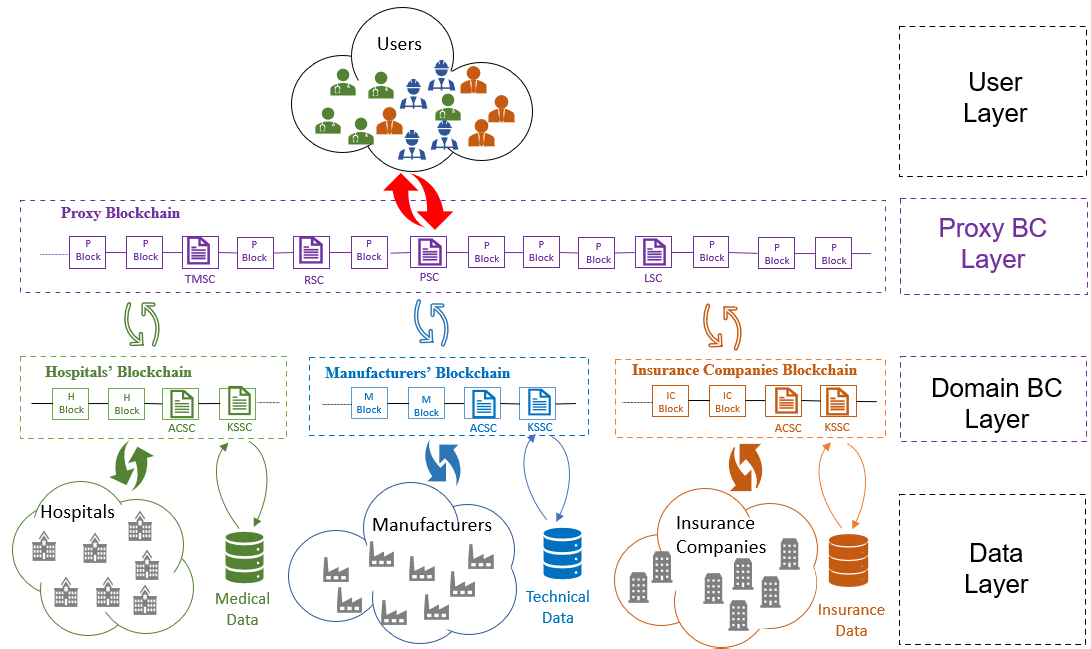
\includegraphics[width=\linewidth]{figures/fig1-architecture.png}\\[-0.1em]
\src{Paper Fig.~1}

\column{0.41\textwidth}
\footnotesize
\begin{itemize}
  \item \textbf{User layer:} one API for people and medical devices.
  \item \textbf{\textcolor{pbc}{Proxy blockchain (PBC)}:} run by \emph{all} stakeholders. It is the single entry point and handles registration, trust lists and the global log.
  \item \textbf{\textcolor{dbc}{Domain blockchains (DBC)}:} one per domain (hospitals, manufacturers, insurers). Each enforces its domain's policy and never talks to users directly.
  \item \textbf{Data layer:} owners keep their data off-chain, ABE-encrypted.
\end{itemize}
\end{columns}

\vspace{0.3em}
\centering
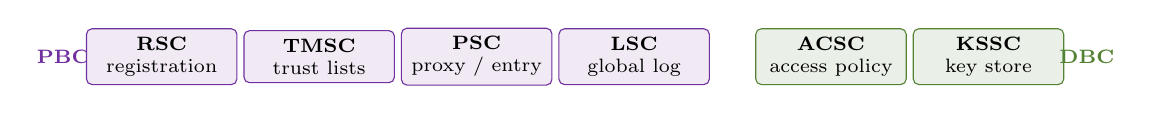
\begin{tikzpicture}[sc/.style={box, minimum height=0.6cm, text width=1.7cm}]
  \node[font=\scriptsize\bfseries, text=pbc] at (-1.25,0) {PBC};
  \node[sc, draw=pbc, fill=pbc!10] at (0,0)    {\textbf{RSC}\\registration};
  \node[sc, draw=pbc, fill=pbc!10] at (2.0,0)  {\textbf{TMSC}\\trust lists};
  \node[sc, draw=pbc, fill=pbc!10] at (4.0,0)  {\textbf{PSC}\\proxy / entry};
  \node[sc, draw=pbc, fill=pbc!10] at (6.0,0)  {\textbf{LSC}\\global log};
  \node[sc, draw=dbc, fill=dbc!12] at (8.5,0)  {\textbf{ACSC}\\access policy};
  \node[sc, draw=dbc, fill=dbc!12] at (10.5,0) {\textbf{KSSC}\\key store};
  \node[font=\scriptsize\bfseries, text=dbc] at (11.75,0) {DBC};
\end{tikzpicture}\\[0.2em]
{\scriptsize Each stakeholder runs one PBC node and one DBC node; all chains are permissioned and use Proof-of-Stake.}
\note{Six smart contracts: four on the proxy chain (RSC, TMSC, PSC, LSC) and two on each domain chain (ACSC, KSSC).}
\end{frame}

% ---------------------------------------------------------------- 5. Trust and temporal roles
\begin{frame}{Trust management and temporal roles}
\begin{columns}[T,onlytextwidth]
\column{0.57\textwidth}
\centering
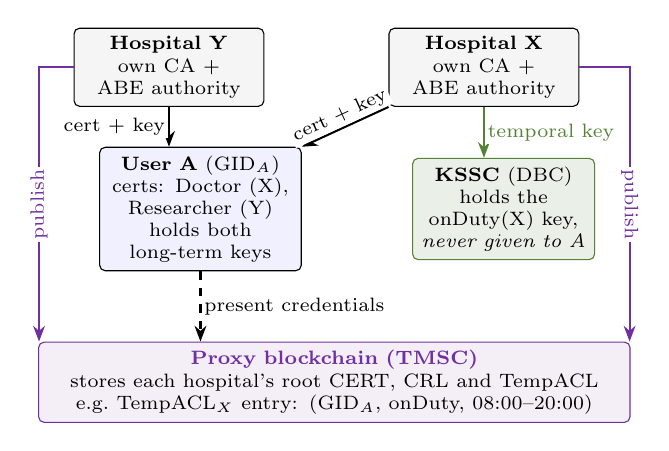
\begin{tikzpicture}[x=1cm, y=1cm, org/.style={box, fill=gray!8, text width=2.2cm}]
  \node[org] (hy) at (0.9,3.9) {\textbf{Hospital Y}\\own CA + ABE authority};
  \node[org] (hx) at (4.9,3.9) {\textbf{Hospital X}\\own CA + ABE authority};
  \node[box, fill=blue!6, text width=2.35cm] (ua) at (1.3,2.1) {\textbf{User A} (GID$_A$)\\certs: Doctor (X),\\Researcher (Y)\\holds both long-term keys};
  \node[box, draw=dbc, fill=dbc!12, text width=2.1cm] (ks) at (5.15,2.1) {\textbf{KSSC} (DBC)\\holds the\\onDuty(X) key,\\\emph{never given to A}};
  \node[box, draw=pbc, fill=pbc!8, text width=7.3cm] (pb) at (3.0,-0.1) {\textbf{\textcolor{pbc}{Proxy blockchain (TMSC)}}\\stores each hospital's root CERT, CRL and TempACL\\e.g.\ TempACL$_X$ entry: (GID$_A$, onDuty, 08:00–20:00)};
  \coordinate (L) at (-0.75,0);
  \coordinate (R) at (6.75,0);
  \draw[->, thick] (hy.south) -- node[lbl, left] {cert + key} (hy.south |- ua.north);
  \draw[->, thick] (hx.south west) -- node[lbl, above, sloped] {cert + key} (ua.north east);
  \draw[->, thick, dbc] (hx.south) -- node[lbl, right] {temporal key} (hx.south |- ks.north);
  \draw[->, thick, pbc] (hy.west) -| node[lbl, text=pbc, rotate=90, pos=0.75] {publish} (L |- pb.north);
  \draw[->, thick, pbc] (hx.east) -| node[lbl, text=pbc, rotate=-90, pos=0.75] {publish} (R |- pb.north);
  \draw[->, thick, dashed] (ua.south) -- node[lbl, right] {present credentials} (ua.south |- pb.north);
\end{tikzpicture}

\column{0.40\textwidth}
\footnotesize
\begin{itemize}
  \item \textbf{No global root CA:} each stakeholder runs its own CA and its own ABE key authority.
  \item \textbf{Trust lists on the PBC:} CA-Admins publish CERT, CRL and TempACL; the TMSC checks credentials against the latest lists.
  \item \textbf{One global ID:} registration (RSC) links a user's certificates, so keys from different authorities combine (Lewko–Waters MA-CP-ABE).
  \item \textbf{Long-term vs.\ temporal roles:} Doctor sits in the certificate, onDuty in the TempACL. A temporal role counts only together with a long-term one.
\end{itemize}
\end{columns}
\note{Paper §III-C5/C6 and §III-D (Figs. 3 and 4). Adding or removing a stakeholder needs consensus of the CA-Admins. The 08:00–20:00 window is our illustrative example.}
\end{frame}

% ---------------------------------------------------------------- 6. Access flow
\begin{frame}{How an access request flows}
\centering
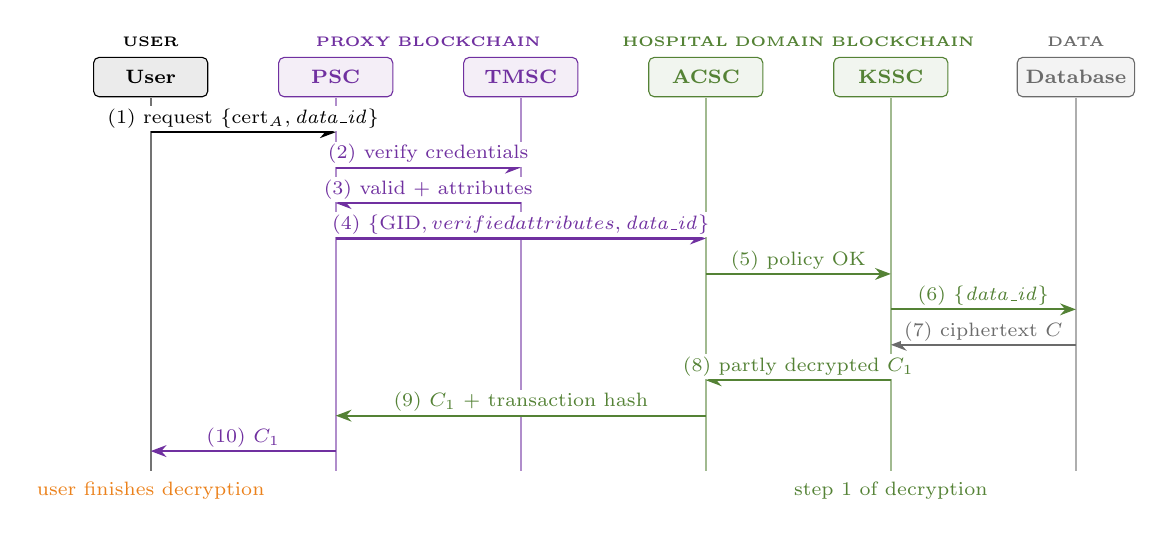
\begin{tikzpicture}[x=1cm, y=1cm]
  \foreach \name/\x/\col in {User/0/black, PSC/2.35/pbc, TMSC/4.7/pbc, ACSC/7.05/dbc, KSSC/9.4/dbc, Database/11.75/datagray} {
    \node[lane, draw=\col, text=\col, fill=\col!8] at (\x,0) {\name};
    \draw[\col!55, thick] (\x,-0.27) -- (\x,-5.0);
  }
  \node[font=\tiny\bfseries]                at (0,0.45)     {USER};
  \node[font=\tiny\bfseries, text=pbc]      at (3.525,0.45) {PROXY BLOCKCHAIN};
  \node[font=\tiny\bfseries, text=dbc]      at (8.225,0.45) {HOSPITAL DOMAIN BLOCKCHAIN};
  \node[font=\tiny\bfseries, text=datagray] at (11.75,0.45) {DATA};
  \seqmsg{0}{2.35}{-0.7}{(1) request $\{\mathrm{cert}_A, \mathit{data\_id}\}$}{black}
  \seqmsg{2.35}{4.7}{-1.15}{(2) verify credentials}{pbc}
  \seqmsg{4.7}{2.35}{-1.6}{(3) valid + attributes}{pbc}
  \seqmsg{2.35}{7.05}{-2.05}{(4) $\{\mathrm{GID}, \text{verified attributes}, \mathit{data\_id}\}$}{pbc}
  \seqmsg{7.05}{9.4}{-2.5}{(5) policy OK}{dbc}
  \seqmsg{9.4}{11.75}{-2.95}{(6) $\{\mathit{data\_id}\}$}{dbc}
  \seqmsg{11.75}{9.4}{-3.4}{(7) ciphertext $C$}{datagray}
  \seqmsg{9.4}{7.05}{-3.85}{(8) partly decrypted $C_1$}{dbc}
  \seqmsg{7.05}{2.35}{-4.3}{(9) $C_1$ + transaction hash}{dbc}
  \seqmsg{2.35}{0}{-4.75}{(10) $C_1$}{pbc}
  \node[font=\scriptsize, text=accent] at (0,-5.25) {user finishes decryption};
  \node[font=\scriptsize, text=dbc] at (9.4,-5.25) {step 1 of decryption};
\end{tikzpicture}

\vspace{0.1em}
\raggedright\footnotesize\textbf{Logging at every hop:} the LSC opens a record at (1) and stores it on the PBC at (10); the ACSC logs on the DBC at (9). $C_1$ is still unreadable without the user's long-term key.
\note{Redrawn from paper Fig. 6. The TMSC checks CERT, CRL and TempACL at (2). The PSC returns the response to the user encrypted with the user's public key.}
\end{frame}

% ---------------------------------------------------------------- 7. Two-step decryption
\begin{frame}{Key idea: split the decryption between the KSSC and the user}
\begin{columns}[T,onlytextwidth]
\column{0.53\textwidth}
\centering
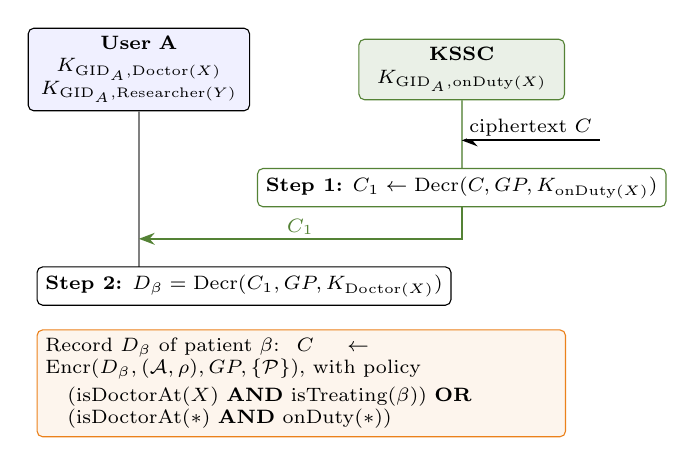
\begin{tikzpicture}[x=1cm, y=1cm]
  \node[box, fill=blue!6, text width=2.6cm] (u) at (0,0) {\textbf{User A}\\$K_{\mathrm{GID}_A,\mathrm{Doctor}(X)}$\\$K_{\mathrm{GID}_A,\mathrm{Researcher}(Y)}$};
  \node[box, draw=dbc, fill=dbc!12, text width=2.4cm] (k) at (4.1,0) {\textbf{KSSC}\\$K_{\mathrm{GID}_A,\mathrm{onDuty}(X)}$};
  \draw[thick, gray] (u.south) -- (0,-2.55);
  \draw[thick, dbc!70] (k.south) -- (4.1,-1.45);
  \draw[->, thick] (5.85,-0.9) -- node[lbl, above] {ciphertext $C$} (4.1,-0.9);
  \node[box, draw=dbc, fill=white] (s1) at (4.1,-1.5) {\textbf{Step 1:} $C_1 \leftarrow \mathrm{Decr}(C, GP, K_{\mathrm{onDuty}(X)})$};
  \draw[->, thick, dbc] (s1.south) |- node[lbl, above, pos=0.75] {$C_1$} (0,-2.15);
  \node[box, fill=white, anchor=west] (s2) at (-1.3,-2.75) {\textbf{Step 2:} $D_\beta = \mathrm{Decr}(C_1, GP, K_{\mathrm{Doctor}(X)})$};
  \node[box, draw=accent, fill=accent!8, text width=6.5cm, align=left, anchor=north west] at (-1.3,-3.3)
    {Record $D_\beta$ of patient $\beta$: \;$C \leftarrow \mathrm{Encr}(D_\beta, (\mathcal{A},\rho), GP, \{\mathcal{P}\})$, with policy\\[2pt]
     \quad(isDoctorAt$(X)$ \textbf{AND} isTreating$(\beta)$) \textbf{OR}\\
     \quad(isDoctorAt$(*)$ \textbf{AND} onDuty$(*)$)};
\end{tikzpicture}\\[0.2em]
\src{Redrawn from paper Fig.~5}

\column{0.44\textwidth}
\footnotesize
\textbf{Why split it?}
\begin{itemize}
  \item \textbf{Revocation is a list update:} temporal keys never reach users, so when the duty ends the hospital only updates its TempACL. No ABE key is revoked or re-issued.
  \item \textbf{The KSSC is not fully trusted:} without the long-term keys it cannot decrypt anything alone.
  \item \textbf{Lighter clients:} the user's device does only the last step.
  \item \textbf{No bypass:} a ‘System’ role added with AND to every policy forces all access through the KSSC.
\end{itemize}
\smallskip
\scriptsize Implemented by splitting Lewko–Waters MA-CP-ABE decryption (Charm library) into a KSSC step and a user step.
\end{columns}
\note{Paper §III-E2 and §V-A4. Only the temporal ABE keys are stored on-chain; their protection relies on the isolation mechanism, and even if leaked they are not enough alone because of the AND policy.}
\end{frame}

% ---------------------------------------------------------------- 8. Results
\begin{frame}{Results: prototype performance}
\scriptsize\textbf{Setup:} private Ethereum (Ganache/Truffle), 6 Solidity contracts, Charm MA-CP-ABE, Docker + Kubernetes; 12-core Ryzen; Proof-of-Stake at $\approx$1000\,tx/s with $\approx$12\,s blocks.

\begin{columns}[T,onlytextwidth]
\column{0.46\textwidth}
\centering
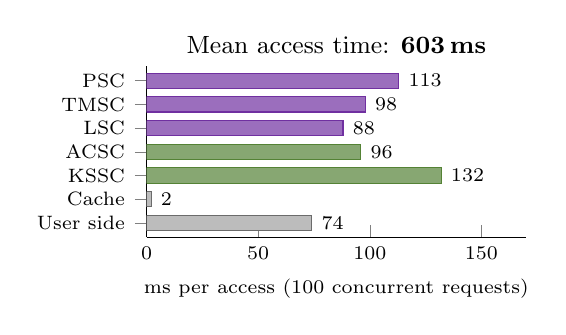
\begin{tikzpicture}
\begin{axis}[
    xbar, bar width=5.5pt, width=6.4cm, height=3.75cm,
    xmin=0, xmax=170, axis x line*=bottom, axis y line*=left,
    symbolic y coords={User side,Cache,KSSC,ACSC,LSC,TMSC,PSC},
    ytick={User side,Cache,KSSC,ACSC,LSC,TMSC,PSC},
    tick label style={font=\scriptsize}, xlabel style={font=\scriptsize},
    xlabel={ms per access (100 concurrent requests)},
    nodes near coords, nodes near coords style={font=\scriptsize},
    enlarge y limits=0.1, bar shift=0pt,
    title={\small Mean access time: \textbf{603\,ms}}, title style={yshift=-5pt},
  ]
  \addplot[fill=pbc!70, draw=pbc] coordinates {(113,PSC) (98,TMSC) (88,LSC)};
  \addplot[fill=dbc!70, draw=dbc] coordinates {(96,ACSC) (132,KSSC)};
  \addplot[fill=datagray!45, draw=datagray] coordinates {(2,Cache) (74,User side)};
\end{axis}
\end{tikzpicture}\\
\src{Paper Table~4: contracts 527\,ms + cache 2\,ms + user 74\,ms}

\column{0.51\textwidth}
\centering
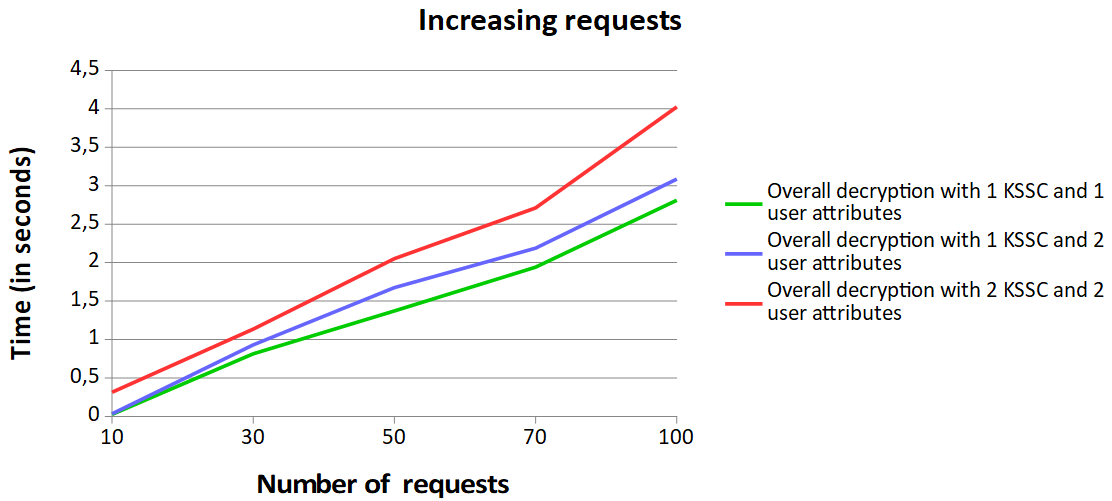
\includegraphics[width=0.86\linewidth]{figures/fig11-requests.png}\\
\src{Paper Fig.~11 (CC BY 4.0)}
\begin{itemize}\scriptsize
  \item About 1\,s at 30 concurrent requests, rising to 3–4\,s at 100.
  \item Decryption time grows with the number of attributes. Overall it is slightly slower than one-step MA-ABE, but the user's share is smaller.
\end{itemize}
\end{columns}

\begin{alertblock}{Security evaluation: an informal argument, under these assumptions}
\scriptsize Isolation holds \,,\, honest majority in every chain \,,\, secure crypto \,,\, uncompromised keys \,,\, polynomially bounded adversary. Measured on one machine, without network delays.
\end{alertblock}
\note{Table 4 values are exact from the paper. The Fig. 11 discrepancy is between the paper's text and its own chart. The authors note that larger-scale studies are needed.}
\end{frame}

% ================================================================ PART II: JANUS, our project, stack, E/F/G

% ---------------------------------------------------------------- 9. JANUS: what it adds
\begin{frame}{JANUS (2023): what it adds on top of HMBC}
\begin{columns}[T,onlytextwidth]
\column{0.43\textwidth}
\centering
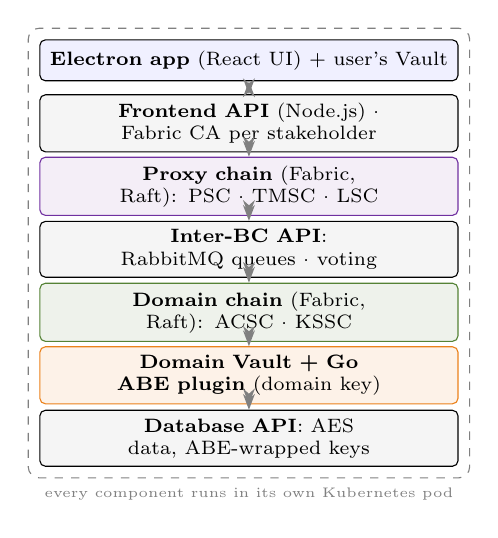
\begin{tikzpicture}[x=1cm, y=1cm, jl/.style={box, text width=5.1cm, minimum height=0.52cm}]
  \node[jl, fill=blue!6]                    (fe) at (0,0)     {\textbf{Electron app} (React UI) + user's Vault};
  \node[jl, fill=gray!8]                    (fa) at (0,-0.8)  {\textbf{Frontend API} (Node.js) · Fabric CA per stakeholder};
  \node[jl, draw=pbc, fill=pbc!8]           (pc) at (0,-1.6)  {\textbf{Proxy chain} (Fabric, Raft): PSC · TMSC · LSC};
  \node[jl, fill=gray!8]                    (ib) at (0,-2.4)  {\textbf{Inter-BC API}: RabbitMQ queues · voting};
  \node[jl, draw=dbc, fill=dbc!10]          (dc) at (0,-3.2)  {\textbf{Domain chain} (Fabric, Raft): ACSC · KSSC};
  \node[jl, draw=accent, fill=accent!10]    (va) at (0,-4.0)  {\textbf{Domain Vault + Go ABE plugin} (domain key)};
  \node[jl, fill=gray!8]                    (db) at (0,-4.8)  {\textbf{Database API}: AES data, ABE-wrapped keys};
  \foreach \a/\b in {fe/fa,fa/pc,pc/ib,ib/dc,dc/va,va/db} \draw[<->, thick, gray] (\a.south) -- (\b.north);
  \node[draw, dashed, gray, rounded corners, fit=(fe)(db), inner sep=4pt] (k8s) {};
  \node[font=\tiny, text=gray, anchor=north] at (k8s.south) {every component runs in its own Kubernetes pod};
\end{tikzpicture}\\[0.1em]
\src{Simplified from JANUS Fig.~5}

\column{0.54\textwidth}
\footnotesize
Same authors with CENSUS S.A., \emph{Applied Sciences} 13(1):566, 2023.
\begin{itemize}
  \item \textbf{Formal model (HMBAC):} sets and relations, with three checks: attribute verification (PBC), authorisation and decryption (DBC).
  \item \textbf{Open-source system:} Fabric 2.4 + Raft, JavaScript contracts, Kubernetes pods.
  \item \textbf{Single access point enforced by crypto:} every policy gets an extra AND with a \emph{domain key} that only the KSSC can derive (in Vault). This realises HMBC's ‘System’ role. Records use AES, with MA-ABE only on the AES keys.
  \item \textbf{Engineering:} RabbitMQ queues with throttling; voting for domains, stakeholders and policies.
  \item \textbf{Evaluation:} attack trees; 2–300 concurrent requests on cloud servers, with linear growth and no failed requests.
\end{itemize}
\end{columns}
\note{JANUS = Malamas, Palaiologos, Kotzanikolaou, Burmester, Glynos, Appl. Sci. 13(1):566, 2023, doi 10.3390/app13010566. Code: github.com/CENSUS/Janus.}
\end{frame}

% ---------------------------------------------------------------- 10. JANUS vs HMBC
\begin{frame}{JANUS vs.\ HMBC: what changed, and why}
\scriptsize
\renewcommand{\arraystretch}{1.2}
\begin{tabular}{@{}>{\bfseries}L{0.14\textwidth} L{0.26\textwidth} L{0.30\textwidth} L{0.27\textwidth}@{}}
\toprule
 & \textbf{HMBC (2020)} & \textbf{JANUS (2023)} & \textbf{Why} \\
\midrule
Platform & private Ethereum (Ganache, Truffle), Proof-of-Stake & Hyperledger Fabric 2.4 with Raft ordering & practical permissioned deployment, reproducible artifact \\
Contracts & 6: RSC, TMSC, PSC, LSC | ACSC, KSSC & 5: no RSC; login via each stakeholder's Fabric CA & identity stays with each stakeholder's CA \\
KSSC key & temporal-role keys (onDuty), never given to users & a \emph{domain} key derived per GID inside Vault & force every decryption through the system \\
Temporal roles & enforced by withholding $K_{\mathrm{onDuty}}$ & user holds $K_{\mathrm{doctor}}$ and $K_{\mathrm{onDuty}}$; duty checked online & \emph{our note:} ending a duty then relies on the online check \\
Key storage & inside the KSSC, behind container isolation & HashiCorp Vault (user side and domain side) & an off-the-shelf secret store \\
Chain to chain & inter-blockchain API + cache & RabbitMQ queues, prioritisation, throttling & avoid congestion and failures \\
Governance & “majority consent”, mechanism unspecified & voting manager with elections and thresholds & concrete joins, leaves and policy changes \\
\bottomrule
\end{tabular}

\vspace{0.5em}
\begin{alertblock}{What JANUS itself leaves open}
\scriptsize Raft tolerates crashes only; Byzantine tolerance is named as future work. Kubernetes/Vault isolation and an honest majority are assumed. No key rotation or epochs are described.
\end{alertblock}
\note{The "Why" column follows JANUS's own motivation, except the temporal-roles row, which is our reading of its Section 4.2.3.}
\end{frame}

% ---------------------------------------------------------------- 11. Our project: RQs
\begin{frame}{Our project: three research questions, answered in order}
\centering
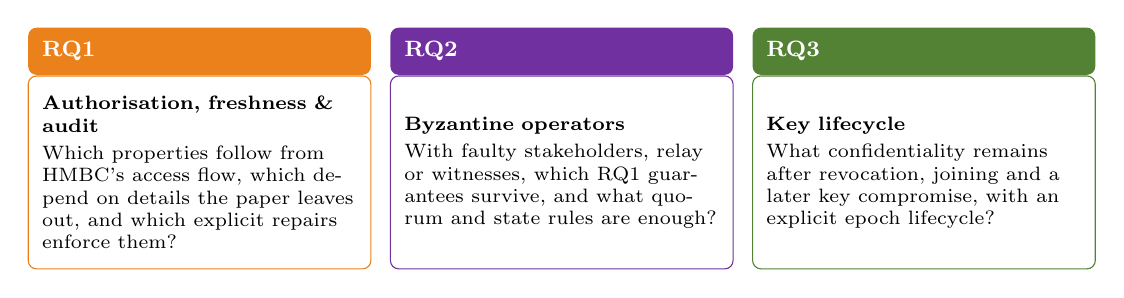
\begin{tikzpicture}[x=1cm, y=1cm,
    card/.style={draw, rounded corners=3pt, text width=4.0cm, align=left, inner sep=5pt, font=\scriptsize, minimum height=2.45cm, anchor=north},
    head/.style={rounded corners=3pt, text width=4.0cm, inner sep=5pt, font=\footnotesize\bfseries, text=white, anchor=south}]
  \foreach \x/\col/\h/\t/\body in {
      0/accent/{RQ1}/{Authorisation, freshness \& audit}/{Which properties follow from HMBC's access flow, which depend on details the paper leaves out, and which explicit repairs enforce them?},
      4.6/pbc/{RQ2}/{Byzantine operators}/{With faulty stakeholders, relay or witnesses, which RQ1 guarantees survive, and what quorum and state rules are enough?},
      9.2/dbc/{RQ3}/{Key lifecycle}/{What confidentiality remains after revocation, joining and a later key compromise, with an explicit epoch lifecycle?}} {
    \node[card, draw=\col] at (\x,0) {\textbf{\t}\\[2pt]\body};
    \node[head, fill=\col] at (\x,0) {\h};
  }
  % timeline
\end{tikzpicture}

\vspace{0.3em}
\raggedright\scriptsize
\textbf{Method:} a paper-derived reconstruction (the authors' code is not available). Every case runs in \textbf{paper-strict}, \textbf{paper-minimal} and \textbf{repaired-e} profiles, plus deliberate \textbf{mutants}; each result is labelled SUPPORTED, SPEC\_GAP, REPAIR\_SUPPORTED, REFUTED or BLOCKED.

\textbf{Team setup:} three modules (ledger, protocol, evaluation) built in parallel on three machines, synchronised through Git and a frozen, hash-pinned interface.
\note{Status as of 2026-10-12: gate E PASS (all 56 catalog rows, ProVerif, three matching sign-offs); the board is at F0. F needs its own plan before any F code; G stays locked until gate F passes.}
\end{frame}

% ---------------------------------------------------------------- 12. Why this direction
\begin{frame}{Why this direction: HMBC's gaps and the surrounding literature}
\scriptsize
\renewcommand{\arraystretch}{1.25}
\begin{tabular}{@{}>{\bfseries}L{0.07\textwidth} L{0.29\textwidth} L{0.32\textwidth} L{0.28\textwidth}@{}}
\toprule
 & \textbf{What HMBC leaves open} & \textbf{What the literature covers} & \textbf{Our angle} \\
\midrule
\textcolor{accent}{RQ1} & Fig.~6 forwards “verified attributes” to the DBC, and nothing binds the DBC grant to the PBC decision. Trust lists are “the latest” with no versions. Outcomes are logged without DBC evidence. & In general, cross-chain messages need a trusted third party (Zamyatin et al., FC 2021). Typed, domain-separated signatures and nonces are standard practice (EIP-712). & An executable, instance-level analysis of HMBC's own flow: paper vs.\ repaired profiles, mutants, ProVerif. \\
\textcolor{pbc}{RQ2} & Security assumes an honest majority and isolation; consensus is just “PoS”; one trusted relay/witness path. & BFT ordering for permissioned chains exists (Sousa, Bessani, Vukolić, DSN 2018). JANUS defers Byzantine tolerance to future work. & Not a consensus swap: which RQ1 guarantees survive one faulty witness under a 3-of-4 quorum, with a trust matrix and a TLC model. \\
\textcolor{dbc}{RQ3} & Revocation is gatekeeping only (withheld keys, list updates). There are no key epochs, and cached plaintext stays usable. & Decentralised MA-ABE (Lewko–Waters, EUROCRYPT 2011); outsourced decryption (Green–Hohenberger–Waters, USENIX Security 2011); revocable, forward-secure MA-ABE schemes (e.g.\ Bkakria et al., 2023). & Measure what a mediated, hierarchical design loses on revocation, joining and compromise; an epoch lifecycle with real ABE, not attribute renaming. \\
\bottomrule
\end{tabular}

\vspace{0.6em}
\tiny\color{datagray} Our (non-exhaustive) literature search found no published instance-level security analysis of HMBC or JANUS. The class-level results above exist and are cited, not claimed as ours.
\end{frame}

% ---------------------------------------------------------------- 13. Tech stack comparison
\begin{frame}{Tech stack: the paper, JANUS, and ours}
\scriptsize
\renewcommand{\arraystretch}{1.18}
\begin{tabular}{@{}>{\bfseries}L{0.13\textwidth} L{0.24\textwidth} L{0.24\textwidth} >{\columncolor{accent!10}}L{0.33\textwidth}@{}}
\toprule
 & \textbf{HMBC paper (2020)} & \textbf{JANUS (2023)} & \textbf{Ours} \\
\midrule
Chains & 2 private Ethereum chains (ganache-cli, Truffle) & Hyperledger Fabric 2.4 & 2 local Anvil chains: PBC (id 18545), DBC (id 28545) \\
Contracts & 6, in Solidity & 5, in JavaScript & 6 in Solidity 0.8.37 + a DecisionVerifier; Foundry 1.8.5 \\
Consensus & Proof-of-Stake ($\approx$1000\,tx/s) & Raft (crash faults only) & none (local dev chains); F adds a 3-of-4 witness quorum \\
Chain to chain & inter-blockchain API + cache & Node.js API + RabbitMQ & untrusted Python relay; EIP-712-signed decisions and receipts checked on-chain \\
ABE & Charm MA-CP-ABE (Python); split decryption simulated & MA-ABE in Go (Vault plugin) + AES & symbolic adapter in RQ1; real Charm / Lewko–Waters only after the G0 gate \\
Secrets & temporal keys in the KSSC, behind container isolation & HashiCorp Vault & off-chain key worker (SQLite intent/send log); contracts hold no secrets \\
Deployment & Docker + Kubernetes & Kubernetes pods, Electron/React, Fabric CA & plain processes on laptops; JSON-Schema interface; Git \\
Evaluation & latency, attribute scaling & attack trees, cloud benchmarks & Forge tests + mutants, Python oracle (pytest), ProVerif 2.05; TLA+/TLC for F/G \\
\bottomrule
\end{tabular}
\note{Python 3.13 with eth-account 0.14, jsonschema 4.26 and pytest 9.0 (uv lockfile) on the off-chain side. Anvil chains run with interval mining (one block per second).}
\end{frame}

% ---------------------------------------------------------------- 14. Why this stack
\begin{frame}{Why this stack: what we keep, and what we change}
\begin{columns}[T,onlytextwidth]
\column{0.47\textwidth}
\centering
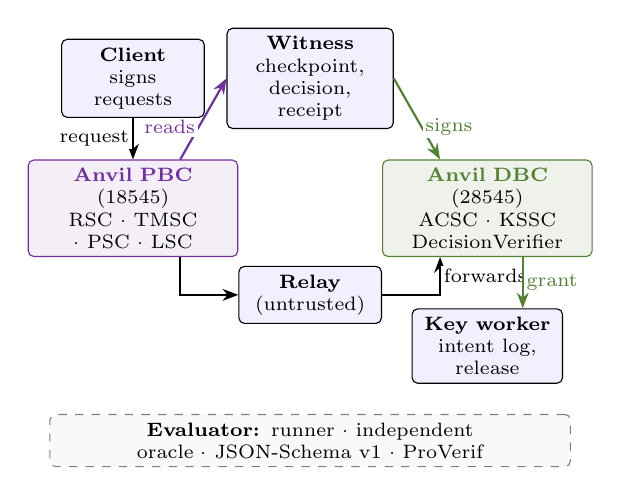
\begin{tikzpicture}[x=1cm, y=1cm, svc/.style={box, fill=blue!6, text width=1.95cm}]
  \node[box, draw=pbc, fill=pbc!8, text width=2.45cm] (pbc) at (0,2.1) {\textbf{\textcolor{pbc}{Anvil PBC}} (18545)\\RSC · TMSC · PSC · LSC};
  \node[box, draw=dbc, fill=dbc!10, text width=2.45cm] (dbc) at (4.5,2.1) {\textbf{\textcolor{dbc}{Anvil DBC}} (28545)\\ACSC · KSSC\\DecisionVerifier};
  \node[svc, text width=1.6cm] (cl) at (0,3.75) {\textbf{Client}\\signs requests};
  \node[svc, text width=1.9cm] (wi) at (2.25,3.75) {\textbf{Witness}\\checkpoint, decision, receipt};
  \node[svc, text width=1.6cm] (re) at (2.25,1.0) {\textbf{Relay}\\(untrusted)};
  \node[svc, text width=1.7cm] (wo) at (4.5,0.35) {\textbf{Key worker}\\intent log, release};
  \draw[->, thick] (cl) -- node[lbl, left] {request} (pbc);
  \draw[->, thick, pbc] (pbc.north) ++(0.6,0) -- node[lbl, left, pos=0.4] {reads} (wi.west);
  \draw[->, thick, dbc] (wi.east) -- node[lbl, right, pos=0.6] {signs} ($(dbc.north)+(-0.6,0)$);
  \draw[->, thick] (pbc.south) ++(0.6,0) |- (re.west);
  \draw[->, thick] (re.east) -| node[lbl, right, pos=0.75] {forwards} ($(dbc.south)+(-0.6,0)$);
  \draw[->, thick, dbc] ($(dbc.south)+(0.45,0)$) -- node[lbl, right] {grant} ($(wo.north)+(0.45,0)$);
  \node[box, dashed, draw=gray, fill=gray!5, text width=6.4cm] (ev) at (2.25,-0.85) {\textbf{Evaluator:} runner · independent oracle · JSON-Schema v1 · ProVerif};
\end{tikzpicture}\\[0.1em]
\src{Python services (blue) and two Solidity ledgers}

\column{0.50\textwidth}
\footnotesize
\textbf{\textcolor{okgreen}{Kept}}
\begin{itemize}\setlength{\itemsep}{1pt}
  \item EVM + Solidity, with the paper's six contracts and callers (HMBC's own platform).
  \item Separate proxy and domain chains.
  \item Charm's Lewko–Waters MA-CP-ABE for RQ3 (the paper's library).
  \item Secrets off-chain in a key service (JANUS's Vault idea, kept minimal).
\end{itemize}
\textbf{\textcolor{badred}{Changed on purpose}}
\begin{itemize}\setlength{\itemsep}{1pt}
  \item Foundry/Anvil, not Ganache/Truffle (both sunset in 2023).
  \item No Fabric, Kubernetes or Vault: we study HMBC2020's design, at laptop scale.
  \item Untrusted relay: EIP-712-signed requests and decisions, checked on-chain.
  \item No consensus claims; RQ2 studies witness quorums.
\end{itemize}
\end{columns}
\end{frame}

% ================================================================ PHASE E (RQ1): gaps, method, results, gate
% Source of every number below: evaluation/reports/RQ1-E.md (69dabfba..), communication/GATES.md (E section,
% decision of 2026-10-12) and the gate run evaluation/evidence/e3/gate-run-20261012/ on origin/agent-1.

% % ---------------------------------------------------------------- E-1. Where we are
% \begin{frame}{Phase E (RQ1): where we are}
% \begin{center}
% \footnotesize\itshape
% RQ1: which authorization, trust-freshness and audit properties \emph{follow} from HMBC's access flow,\\
% which \emph{depend} on details the paper leaves out, and which explicit \emph{repairs} enforce them?
% \end{center}

% \vspace{-0.2em}
% \centering
% \begin{tikzpicture}[x=1cm, y=1cm,
%     ph/.style={draw, rounded corners=3pt, text width=2.0cm, align=center, inner sep=3pt, font=\scriptsize, minimum height=1.75cm, execute at begin node={\hyphenpenalty=10000\exhyphenpenalty=10000}}]
%   \foreach \i/\name/\when/\body/\col/\tint in {
%       0/{E0 · Foundation}/{6–8 Oct}/{interface and 56-row catalog frozen \emph{before} any run}/okgreen/8,
%       1/{E1 · Legit flow}/{8 Oct}/{9/9 integrated controls in all 3 profiles}/okgreen/8,
%       2/{E2 · Attack slices}/{9–11 Oct}/{10 slices, each frozen, run live on two chains, reviewed}/okgreen/8,
%       3/{E3 · Gate E}/{12 Oct}/{one command: 56/56 rows + ProVerif \textbf{PASS}}/okgreen/22,
%       4/{F · RQ2}/{next}/{Byzantine witnesses: 4 signers, quorum 3}/accent/10,
%       5/{G · RQ3}/{later}/{key lifecycle with real MA-ABE}/datagray/6} {
%     \node[ph, draw=\col, fill=\col!\tint] (p\i) at (\i*2.36,0) {\textbf{\name}\\[-1pt]{\tiny\color{datagray}\when}\\[2pt]\body};
%   }
%   \foreach \i [evaluate=\i as \j using int(\i+1)] in {0,...,4} \draw[->, thick, gray] (p\i) -- (p\j);
%   \node[font=\scriptsize\bfseries, text=accent, anchor=north] at ($(p3.south)!0.5!(p4.south)+(0,-0.05)$) {$\blacktriangle$ we are here};
% \end{tikzpicture}

% \vspace{0.6em}
% \begin{tikzpicture}[x=1cm, y=1cm, every node/.append style={minimum height=1.85cm, font=\footnotesize, execute at begin node={\hyphenpenalty=10000\exhyphenpenalty=10000}}]
%   \node[stat=okgreen] at (0,0)     {{\Large\bfseries 56/56}\\[2pt]catalog rows matched their frozen expected result};
%   \node[stat=accent]  at (3.55,0)  {{\Large\bfseries 20 of 32}\\[2pt]paper-profile rows depend on a detail the paper leaves open};
%   \node[stat=dbc]     at (7.1,0)   {{\Large\bfseries 19 of 24}\\[2pt]repaired-e rows where our explicit check enforces the property};
%   \node[stat=datagray] at (10.65,0) {{\Large\bfseries 0}\\[2pt]HMBC ``exploits'' claimed: the gaps are spec dependencies};
% \end{tikzpicture}

% \vspace{0.6em}
% {\footnotesize \textbf{Gate E PASS} recorded on 12 Oct 2026, after three matching sign-offs. Phase F is next.}
% \note{Gate E PASS was recorded on 12 Oct 2026 (communication/GATES.md, three matching ACKs A1-0085, S2-0023, S3-0024). The other 5 repaired-e rows are controls (receipt signature controls, the receipt positive control, the wrong-issuer baseline). The 20 paper SPEC_GAP rows are 10 attack schedules in two paper profiles.}
% \end{frame}

% ---------------------------------------------------------------- E-2. The research gaps
\begin{frame}{The gaps: what HMBC's access flow leaves unspecified}
\begin{columns}[T,onlytextwidth]
\column{0.50\textwidth}
\centering
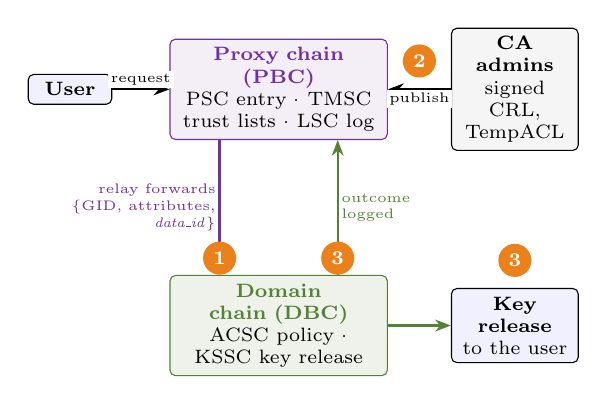
\begin{tikzpicture}[x=1cm, y=1cm,
    gap/.style={circle, fill=accent, text=white, font=\scriptsize\bfseries, inner sep=1.2pt, minimum size=0.42cm}]
  \node[box, fill=blue!6, text width=0.85cm] (u) at (0,0) {\textbf{User}};
  \node[box, draw=pbc, fill=pbc!8, text width=2.55cm, minimum height=1.05cm] (pbc) at (2.65,0)
       {\textbf{\textcolor{pbc}{Proxy chain (PBC)}}\\PSC entry · TMSC trust lists · LSC log};
  \node[box, fill=gray!8, text width=1.4cm] (ca) at (5.65,0) {\textbf{CA admins}\\signed CRL, TempACL};
  \node[box, draw=dbc, fill=dbc!10, text width=2.55cm, minimum height=1.05cm] (dbc) at (2.65,-3.0)
       {\textbf{\textcolor{dbc}{Domain chain (DBC)}}\\ACSC policy · KSSC key release};
  \node[box, fill=blue!6, text width=1.4cm] (rel) at (5.65,-3.0) {\textbf{Key release}\\to the user};
  \draw[->, thick] (u) -- node[lbl, above, font=\tiny] {request} (pbc);
  \draw[->, thick] (ca) -- node[lbl, below, font=\tiny] {publish} (pbc);
  \draw[->, thick, pbc] ($(pbc.south)+(-0.75,0)$) -- node[lbl, left, align=right, text width=1.9cm, font=\tiny] {relay forwards\\$\{$GID, attributes,\\\textit{data\_id}$\}$} ($(dbc.north)+(-0.75,0)$);
  \draw[->, thick, dbc] ($(dbc.north)+(0.75,0)$) -- node[lbl, right, align=left, font=\tiny] {outcome\\logged} ($(pbc.south)+(0.75,0)$);
  \draw[->, thick, dbc] (dbc) -- (rel);
  \node[gap] at ($(pbc.south)+(-0.75,-1.5)$) {1};
  \node[gap] at ($(pbc.east)!0.5!(ca.west)+(0,0.36)$) {2};
  \node[gap] at ($(pbc.south)+(0.75,-1.5)$) {3};
  \node[gap] at ($(rel.north)+(0,0.35)$) {3};
\end{tikzpicture}\\[0.2em]
\src{Simplified from paper Fig.~6; circles mark the gaps}

\column{0.47\textwidth}
\footnotesize
\renewcommand{\arraystretch}{1.25}
\begin{tabular}{@{}c L{0.88\linewidth}@{}}
\gapn{1} & \textbf{RQ1-01 decision provenance.} The DBC sees a tuple, not the PBC's decision. Nothing says \emph{who} it is for, \emph{which chain} it targets, \emph{when} it expires, or that it is \emph{new}. \\
\gapn{2} & \textbf{RQ1-02 trust-anchor freshness.} Lists are ``the latest'', with no version or expiry. Nothing says \emph{when} a revocation must reach the DBC. \\
\gapn{3} & \textbf{RQ1-03 audit correspondence.} An outcome can be logged without DBC evidence. The paper is silent on a crash between key release and logging. \\
\end{tabular}

\end{columns}
\note{Source map: 37 paper passages (S01-S37) and 41 recorded completions (A01-A41) in interfaces/v1. Gap 1 is A02/A14/A19/A25, gap 2 A09/A17/A20/A22, gap 3 A03/A11/A12/A26.}
\end{frame}

% ---------------------------------------------------------------- E-3. Method
\begin{frame}{Method: the paper and our repair on one frozen catalog}
\begin{columns}[T,onlytextwidth]
\column{0.40\textwidth}
\footnotesize\textbf{Four profiles of the same six contracts}\\[0.3em]
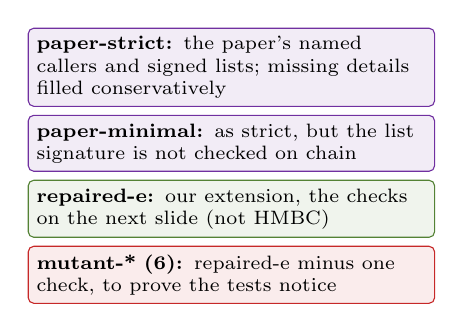
\begin{tikzpicture}[x=1cm, y=1cm, every node/.append style={execute at begin node={\hyphenpenalty=10000\exhyphenpenalty=10000}}]
  \node[prof=pbc, anchor=north west] (a) at (0,0) {\textbf{paper-strict:} the paper's named callers and signed lists; missing details filled conservatively};
  \node[prof=pbc, anchor=north west] (b) at ($(a.south west)+(0,-0.1)$) {\textbf{paper-minimal:} as strict, but the list signature is not checked on chain};
  \node[prof=dbc, anchor=north west] (c) at ($(b.south west)+(0,-0.1)$) {\textbf{repaired-e:} our extension, the checks on the next slide (not HMBC)};
  \node[prof=badred, anchor=north west] (d) at ($(c.south west)+(0,-0.1)$) {\textbf{mutant-* (6):} repaired-e minus one check, to prove the tests notice};
\end{tikzpicture}

\vspace{0.4em}
\textbf{Each row gets one class}\\[0.1em]
\scriptsize
\renewcommand{\arraystretch}{1.15}
\begin{tabular}{@{}l L{0.60\linewidth}@{}}
\cSup & follows from the paper (as reconstructed) \\
\cGap & depends on a detail the paper leaves open \\
\cRep & our repair enforces it \\
\cBlk & cannot be decided from the paper \\
\end{tabular}

\column{0.57\textwidth}
\footnotesize\textbf{How each result is produced}\\[0.3em]
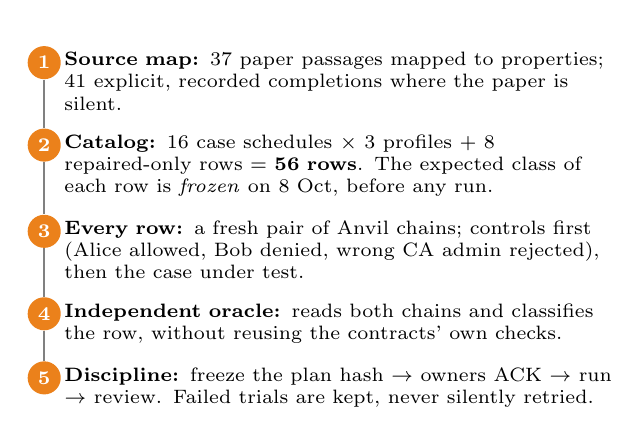
\begin{tikzpicture}[x=1cm, y=1cm,
    num/.style={circle, fill=accent, text=white, font=\scriptsize\bfseries, inner sep=1pt, minimum size=0.42cm},
    st/.style={text width=7.0cm, align=left, font=\scriptsize, anchor=north west, inner sep=0pt, execute at begin node={\hyphenpenalty=10000\exhyphenpenalty=10000}}]
  \node[inner sep=0pt, minimum size=0pt] (t-1) at (0.4,0.3) {};
  \foreach \i/\t in {
      0/{\textbf{Source map:} 37 paper passages mapped to properties; 41 explicit, recorded completions where the paper is silent.},
      1/{\textbf{Catalog:} 16 case schedules $\times$ 3 profiles + 8 repaired-only rows = \textbf{56 rows}. The expected class of each row is \emph{frozen} on 8 Oct, before any run.},
      2/{\textbf{Every row:} a fresh pair of Anvil chains; controls first (Alice allowed, Bob denied, wrong CA admin rejected), then the case under test.},
      3/{\textbf{Independent oracle:} reads both chains and classifies the row, without reusing the contracts' own checks.},
      4/{\textbf{Discipline:} freeze the plan hash $\rightarrow$ owners ACK $\rightarrow$ run $\rightarrow$ review. Failed trials are kept, never silently retried.}} {
    \pgfmathtruncatemacro{\prev}{\i-1}
    \node[st] (t\i) at ($(t\prev.south west)+(0,-0.3)$) {\t};
    \node[num, anchor=north] (n\i) at ($(t\i.north west)+(-0.25,0.08)$) {\the\numexpr\i+1\relax};
  }
  \foreach \i [evaluate=\i as \j using int(\i+1)] in {0,...,3} \draw[gray, thick] (n\i) -- (n\j);
\end{tikzpicture}
\end{columns}
\note{Catalog: interfaces/v1/scenarios/e0_cases.json (48 rows = 16 schedules x 3 profiles) plus e0_supplement_cases.json (8 repaired-e rows). Positive controls: e_positive.json. Interface v1 FREEZE f700292e.. on 2026-10-08.}
\end{frame}

% ---------------------------------------------------------------- E-4. What repaired-e adds
\begin{frame}{What we built: the repaired-e profile}
\centering
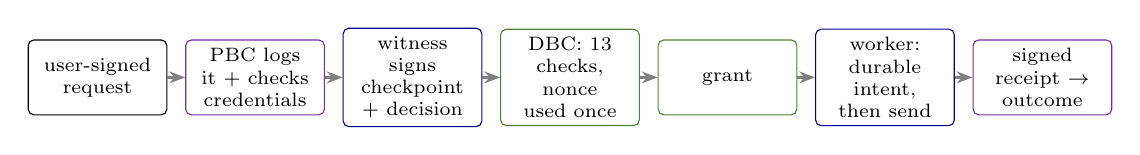
\begin{tikzpicture}[x=1cm, y=1cm, st/.style={box, text width=1.55cm, minimum height=0.95cm, fill=white}]
  \foreach \i/\t/\col in {0/{user-signed request}/black, 1/{PBC logs it + checks credentials}/pbc, 2/{witness signs checkpoint + decision}/blue!60!black, 3/{DBC: 13 checks, nonce used once}/dbc, 4/{grant}/dbc, 5/{worker: durable intent, then send}/blue!60!black, 6/{signed receipt $\to$ outcome}/pbc} {
    \node[st, draw=\col] (s\i) at (\i*2.0,0) {\t};
  }
  \foreach \i [evaluate=\i as \j using int(\i+1)] in {0,...,5} \draw[->, thick, gray] (s\i) -- (s\j);
\end{tikzpicture}

\vspace{0.5em}
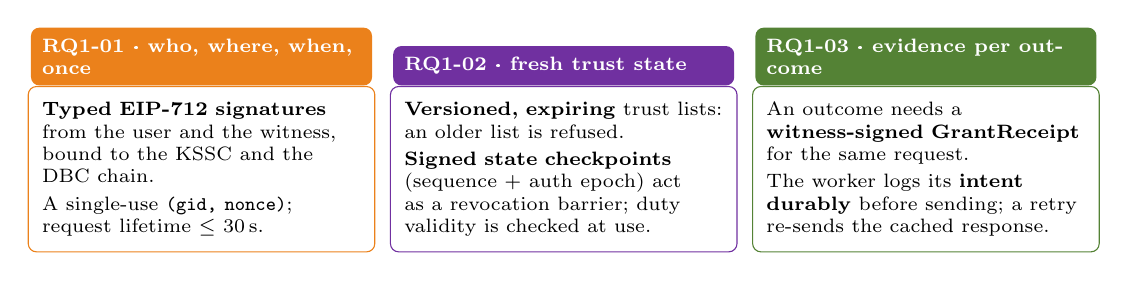
\begin{tikzpicture}[x=1cm, y=1cm, cw/.style={text width=4.05cm, minimum height=2.1cm, execute at begin node={\hyphenpenalty=10000\exhyphenpenalty=10000}}, hw/.style={text width=4.05cm, font=\scriptsize\bfseries}]
  \node[pcard=accent, cw] at (0,0) {%
    \textbf{Typed EIP-712 signatures} from the user and the witness, bound to the KSSC and the DBC chain.\\[2pt]
    A single-use \texttt{(gid, nonce)}; request lifetime $\le$ 30\,s.};
  \node[phead=accent, hw] at (0,0) {RQ1-01 · who, where, when, once};
  \node[pcard=pbc, cw] at (4.6,0) {%
    \textbf{Versioned, expiring} trust lists: an older list is refused.\\[2pt]
    \textbf{Signed state checkpoints} (sequence + auth epoch) act as a revocation barrier; duty validity is checked at use.};
  \node[phead=pbc, hw] at (4.6,0) {RQ1-02 · fresh trust state};
  \node[pcard=dbc, cw] at (9.2,0) {%
    An outcome needs a \textbf{witness-signed GrantReceipt} for the same request.\\[2pt]
    The worker logs its \textbf{intent durably} before sending; a retry re-sends the cached response.};
  \node[phead=dbc, hw] at (9.2,0) {RQ1-03 · evidence per outcome};
\end{tikzpicture}

\vspace{0.45em}
{\scriptsize\textbf{DecisionVerifier on the DBC: 13 checks in a fixed order} (colours as above; step 12 is for RQ3)}\\[0.25em]
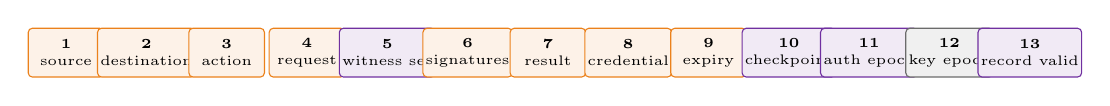
\begin{tikzpicture}[x=1cm, y=1cm]
  \foreach \i/\t/\col in {1/source/accent, 2/destination/accent, 3/action/accent, 4/request/accent, 5/witness set/pbc, 6/signatures/accent, 7/result/accent, 8/credential/accent, 9/expiry/accent, 10/checkpoint/pbc, 11/auth epoch/pbc, 12/key epoch/datagray, 13/record valid/pbc} {
    \node[dv=\col, minimum width=0.96cm] at (\i*1.02,0) {\textbf{\i}\\\t};
  }
\end{tikzpicture}\\[0.1em]
{\scriptsize A certificate with several defects always gets the same error code. Contracts hold no secrets.}
\note{repaired-e is a project extension, not HMBC. DecisionVerifier.sol header fixes the 13 steps; step 12 (key epoch) is reserved for G. Six mutants each remove one check: destination binding (1), state barrier (2), record freshness (4), nonce (8), version monotonicity (16), receipt binding (32).}
\end{frame}

% ---------------------------------------------------------------- E-5. E01 results
\begin{frame}{Results RQ1-01: decision provenance and replay}
\scriptsize
\renewcommand{\arraystretch}{1.22}
\begin{tabular}{@{}L{0.27\textwidth} L{0.33\textwidth} L{0.37\textwidth}@{}}
\toprule
\textbf{The relay\ldots} & \textbf{paper-strict / paper-minimal} & \textbf{repaired-e} \\
\midrule
replays an identical accepted request & \cSup\ rejected: \code{REPLAY}\textsuperscript{$*$} & \cRep\ rejected: \code{REPLAY} \\
swaps the subject (GID) & \cGap\ granted; response goes to the swapped subject & \cRep\ \code{WRONG\_SUBJECT}, step 4 \\
forges a tuple with no PBC request & \cGap\ granted & \cRep\ \code{BAD\_SIGNATURE}, step 6 \\
replays it under a new reference & \cGap\ a second grant & \cRep\ \code{REPLAY}: grant already exists \\
reuses a nonce on a different request & -- (the paper has no nonce) & \cRep\ \code{REPLAY}: nonce already used \\
delivers deployment B's tuple to A & \cGap\ A grants it & \cRep\ \code{WRONG\_DESTINATION}, step 1 \\
delivers it exactly at the request's expiry & \cGap\ granted at that instant & \cRep\ \code{EXPIRED}, step 9 (at equality) \\
\bottomrule
\end{tabular}

\vspace{0.6em}
\begin{columns}[T,onlytextwidth]
\column{0.62\textwidth}
\begin{alertblock}{What it means}
\scriptsize In the paper profiles the DBC grants \emph{any} well-formed tuple the configured relay forwards. Repaired-e rejects each attack at a named verifier step, and Alice's legitimate access still succeeds in every row.
\end{alertblock}
\column{0.35\textwidth}
\tiny\color{datagray}
\textsuperscript{$*$}Only because our grant id is deterministic (a recorded completion), not because the paper has a nonce.\\[3pt]
The relay attacks use a misbehaving relay, which HMBC's isolation assumption excludes.
\end{columns}
\note{Catalog rows 10-22 and 51-56. Gate run E-gate-20261012: all 19 E01 rows PASS with their frozen class and code. The relay stress rows (13-22, 51-53) are outside A01 (secure isolation): specification dependencies, not exploits.}
\end{frame}

% ---------------------------------------------------------------- E-6. E02 results + window
\begin{frame}{Results RQ1-02: trust-anchor freshness and the revocation window}
\begin{columns}[T,onlytextwidth]
\column{0.56\textwidth}
\scriptsize
\renewcommand{\arraystretch}{1.3}
\begin{tabular}{@{}L{0.30\linewidth} L{0.32\linewidth} L{0.32\linewidth}@{}}
\toprule
\textbf{Case} & \textbf{paper profiles} & \textbf{repaired-e} \\
\midrule
CA admin updates another issuer's list & \cSup\ \code{UNAUTHORIZED\_CALLER} (baseline, not a repair) & \cSup\ same \\
an older signed CRL is re-installed & \cGap\ accepted: a \textbf{revoked credential is un-revoked} & \cRep\ \code{STALE\_ANCHOR} \\
revoked; decision used \emph{before} the DBC sees a new checkpoint & \cGap\ accepted & \cRep\ accepted on purpose, inside the bounded window \\
revoked; decision used \emph{after} it & \cGap\ still accepted: there is no barrier & \cRep\ \code{STALE\_STATE} \\
duty ended at delivery & \cGap\ granted at that instant & \cRep\ \code{EXPIRED} (step 13) \\
\bottomrule
\end{tabular}

\column{0.41\textwidth}
\centering
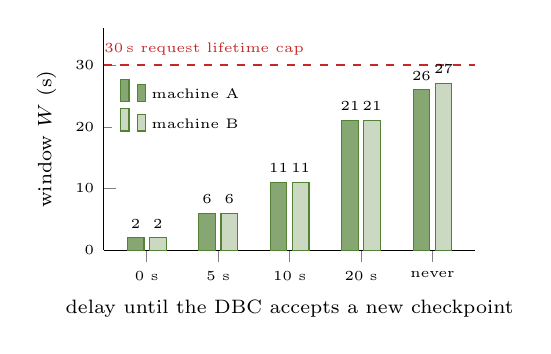
\begin{tikzpicture}
\begin{axis}[
    ybar, bar width=6pt, width=6.3cm, height=4.4cm,
    ymin=0, ymax=36, axis x line*=bottom, axis y line*=left,
    symbolic x coords={0 s,5 s,10 s,20 s,never},
    xtick=data, enlarge x limits=0.15,
    xlabel={delay until the DBC accepts a new checkpoint},
    ylabel={window $W$ (s)},
    tick label style={font=\tiny}, label style={font=\scriptsize},
    nodes near coords, nodes near coords style={font=\tiny},
    legend style={font=\tiny, at={(0.02,0.80)}, anchor=north west, draw=none, fill=white},
    legend cell align=left,
  ]
  \addplot[fill=dbc!70, draw=dbc] coordinates {(0 s,2) (5 s,6) (10 s,11) (20 s,21) (never,26)};
  \addplot[fill=dbc!30, draw=dbc] coordinates {(0 s,2) (5 s,6) (10 s,11) (20 s,21) (never,27)};
  \draw[dashed, badred, thick] (rel axis cs:0,0.833) -- (rel axis cs:1,0.833) node[pos=0.27, above, font=\tiny, text=badred] {30\,s request lifetime cap};
  \legend{machine A, machine B}
\end{axis}
\end{tikzpicture}\\
\scriptsize
\textbf{repaired-e:} $W = \min(\text{checkpoint delay}, \text{lifetime left}) \le 30$\,s\\[1pt]
\textbf{paper-strict:} no bound; still grantable 65\,s later\\[2pt]
\src{owner measurement, 1 trial per delay; not the gate run}
\end{columns}
\note{Rows 36-50 of the gate run. The window chart is the owner measurement A1-0046 (machine A) and A2-0026 (machine B), cited under decision A1-0081; the integrated gate run did not measure a window. The paper pre- and post-barrier rows are one execution.}
\end{frame}

% ---------------------------------------------------------------- E-7. E03 results
\begin{frame}{Results RQ1-03: audit correspondence and crash recovery}
\begin{columns}[T,onlytextwidth]
\column{0.60\textwidth}
\scriptsize
\renewcommand{\arraystretch}{1.3}
\begin{tabular}{@{}L{0.30\linewidth} L{0.30\linewidth} L{0.34\linewidth}@{}}
\toprule
\textbf{Case} & \textbf{paper profiles} & \textbf{repaired-e} \\
\midrule
same outcome reported twice & \cSup\ \code{REPLAY} & \cRep\ \code{REPLAY} \\
relay drops the outcome & \cSup\ request stays PENDING, visibly & \cRep\ same, plus durable worker evidence \\
outcome fabricated, no grant exists & \cGap\ recorded & \cRep\ \code{WRONG\_PROFILE}: needs a receipt \\
receipt names another request, GID or record & -- (no receipts) & \cRep\ \code{WRONG\_SUBJECT}, nothing recorded \\
worker crashes after intent / after send & \cBlk\ the paper is silent on durability & \cRep\ cached response re-sent: one grant, one outcome \\
\bottomrule
\end{tabular}

\column{0.37\textwidth}
\centering
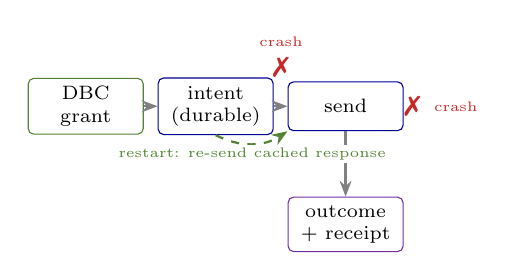
\begin{tikzpicture}[x=1cm, y=1cm, ev/.style={box, text width=1.25cm, minimum height=0.62cm, fill=white}]
  \node[ev, draw=dbc] (g) at (0,0) {DBC grant};
  \node[ev, draw=blue!60!black] (i) at (1.65,0) {intent (durable)};
  \node[ev, draw=blue!60!black] (s) at (3.3,0) {send};
  \node[ev, draw=pbc] (o) at (3.3,-1.5) {outcome + receipt};
  \draw[->, thick, gray] (g) -- (i);
  \draw[->, thick, gray] (i) -- (s);
  \draw[->, thick, gray] (s) -- (o);
  \node[text=badred, font=\bfseries] at (2.48,0.5) {\ding{55}};
  \node[text=badred, font=\bfseries] at (4.15,0.0) {\ding{55}};
  \node[font=\tiny, text=badred] at (2.48,0.82) {crash};
  \node[font=\tiny, text=badred, anchor=west] at (4.3,0.0) {crash};
  \draw[->, thick, dbc, dashed] (i.south) to[bend right=30] node[lbl, below, font=\tiny, text=dbc] {restart: re-send cached response} (s.south west);
\end{tikzpicture}\\[0.4em]
\begin{itemize}\scriptsize
  \item Before the grant expires: the \emph{same} response again, no second capability.
  \item After it expires: \code{EXPIRED}, nothing changes.
  \item A grant is permission to release, \textbf{not proof of delivery}: delivery stays ``unknown'', and we report it that way.
\end{itemize}
\end{columns}

\vspace{0.4em}
\raggedright\tiny\color{datagray}
The four paper crash rows are recorded as ``BLOCKED / decided SPEC\_GAP, unproved'': never a pass, never a finding. Crash points are logical process deaths, not power loss. The receipt-substitution rows use a deliberately deviating test witness.
\note{Dropped outcome: only local durable worker evidence is unconditional; PBC reconciliation needs eventual delivery and an honest reporter. Crash rows: D47. Receipt binding rows 29-31 use the TEST-ONLY deviating witness (A40); rows 32-35 are signature and positive controls (SUPPORTED).}
\end{frame}

% ---------------------------------------------------------------- E-8. Sensitivity: mutants + ProVerif
\begin{frame}{Are the checks real? Mutants and a formal model}
\begin{columns}[T,onlytextwidth]
\column{0.53\textwidth}
\footnotesize\textbf{Remove one check, and something must fail}\\[0.3em]
\scriptsize
\renewcommand{\arraystretch}{1.22}
\begin{tabular}{@{}L{0.26\linewidth} L{0.29\linewidth} L{0.39\linewidth}@{}}
\toprule
\textbf{Mutant} & \textbf{Ledger test that fails} & \textbf{Gate row that hits the guard} \\
\midrule
no nonce & nonce reuse across requests & same nonce: \code{REPLAY} \\
no receipt binding & receipt field swap & receipt $\times$3: \code{WRONG\_SUBJECT} \\
no state barrier & revocation barrier & post-barrier: \code{STALE\_STATE} \\
no record freshness & duty ended at delivery & expired duty: \code{EXPIRED} \\
no version order & stale CRL / TempACL replay & rollback: \code{STALE\_ANCHOR} \\
no destination binding & request field swap; ProVerif & -- (step 1 fires first) \\
\bottomrule
\end{tabular}\\[0.4em]

\column{0.44\textwidth}
\footnotesize\textbf{ProVerif: does each grant match the approvals?}\\[0.3em]
\centering
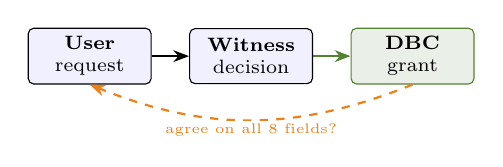
\begin{tikzpicture}[x=1cm, y=1cm, ev/.style={box, text width=1.35cm, minimum height=0.7cm}]
  \node[ev, fill=blue!6] (u) at (0,0) {\textbf{User}\\request};
  \node[ev, fill=blue!6] (w) at (2.05,0) {\textbf{Witness}\\decision};
  \node[ev, draw=dbc, fill=dbc!12] (g) at (4.1,0) {\textbf{DBC}\\grant};
  \draw[->, thick] (u) -- (w);
  \draw[->, thick, dbc] (w) -- (g);
  \draw[->, thick, accent, dashed] (g.south) to[bend left=22] node[lbl, below, text=accent, font=\tiny] {agree on all 8 fields?} (u.south);
\end{tikzpicture}\\[0.2em]
\scriptsize
\renewcommand{\arraystretch}{1.15}
\begin{tabular}{@{}L{0.44\linewidth} L{0.22\linewidth} L{0.26\linewidth}@{}}
\toprule
\textbf{Query} & \textbf{repaired} & \textbf{mutant} \\
\midrule
grant agrees with user + witness on all 8 fields & \textcolor{okgreen}{\textbf{true}} & \textcolor{badred}{\textbf{false}}: attack trace \\
other 7 fields agree & \textcolor{okgreen}{true} & \textcolor{okgreen}{true} \\
legitimate grant reachable & \textcolor{okgreen}{yes} & \textcolor{okgreen}{yes} \\
policy-denied grant & \textcolor{okgreen}{unreachable} & \textcolor{okgreen}{unreachable} \\
\bottomrule
\end{tabular}\\[0.3em]
\raggedright\tiny\color{datagray} Symbolic model (perfect signatures, one honest user and witness); no replay, expiry or revocation.
\end{columns}
\note{Criterion 4 is "met on owner, formal and baseline evidence (human decision A1-0080); integrated live mutant matrix not run". The owner rehearsal (agent 1's runner) ran live mutant probes: 5/6 detected; no-destination-binding is not killable by the catalog recipe because step 1 (source binding) fires first. That rehearsal is owner evidence, not the integrated evaluator.}
\end{frame}

% % ---------------------------------------------------------------- E-9. Gate E
% \begin{frame}{Gate E: one command, 56 rows, a recorded verdict}
% \begin{columns}[T,onlytextwidth]
% \column{0.56\textwidth}
% \centering
% \footnotesize\textbf{Every catalog row, coloured by its result}\\[0.4em]
% \begin{tikzpicture}[x=1cm, y=1cm]
%   % groups: paper profiles at x=0.85, repaired-e at x=4.35; pitch 0.26
%   \node[font=\scriptsize\bfseries, text=pbc, anchor=south west] at (0.85,0.4) {paper-strict + paper-minimal};
%   \node[font=\scriptsize\bfseries, text=dbc, anchor=south west] at (4.35,0.4) {repaired-e};
%   \node[font=\scriptsize\bfseries, anchor=east] at (0.7,0.11)  {E01};
%   \node[font=\scriptsize\bfseries, anchor=east] at (0.7,-0.49) {E02};
%   \node[font=\scriptsize\bfseries, anchor=east] at (0.7,-1.09) {E03};
%   % E01: paper 2 SUP + 10 GAP; repaired 7 REP
%   \wcells{0.85}{0}{0}{2}{clsup}  \wcells{0.85}{2}{0}{10}{clgap}
%   \wcells{4.35}{0}{0}{7}{clrep}
%   % E02: paper 2 SUP + 8 GAP; repaired 4 REP + 1 SUP
%   \wcells{0.85}{0}{-0.6}{2}{clsup}  \wcells{0.85}{2}{-0.6}{8}{clgap}
%   \wcells{4.35}{0}{-0.6}{4}{clrep}   \wcells{4.35}{4}{-0.6}{1}{clsup}
%   % E03: paper 4 SUP + 2 GAP + 4 BLK; repaired 8 REP + 4 SUP
%   \wcells{0.85}{0}{-1.2}{4}{clsup}  \wcells{0.85}{4}{-1.2}{2}{clgap}  \wcells{0.85}{6}{-1.2}{4}{clblk}
%   \wcells{4.35}{0}{-1.2}{8}{clrep}   \wcells{4.35}{8}{-1.2}{4}{clsup}
%   % totals
%   \node[font=\tiny, anchor=north west, align=left] at (0.85,-1.5) {32 rows: \textbf{8} supported\\\textbf{20} spec gap · \textbf{4} blocked};
%   \node[font=\tiny, anchor=north west, align=left] at (4.35,-1.5) {24 rows: \textbf{19} repair supported\\\textbf{5} supported (controls)};
% \end{tikzpicture}\\[0.5em]
% \scriptsize
% \cSup\ \ \cGap\ \ \cRep\ \ \cBlk\\[0.5em]
% \raggedright\scriptsize Every gap in the paper profiles has a repaired-e row with an explicit check. In all 56 rows the observed class and error code equal the \textbf{frozen} expectation: 0 refuted, 0 failed.

% \column{0.41\textwidth}
% \footnotesize
% \textbf{The run (12 Oct)}
% \begin{itemize}\scriptsize\setlength{\itemsep}{1pt}
%   \item One command: 56 rows, each on a fresh pair of chains, then the ProVerif re-run.
%   \item 4,749\,s (1.3\,h), 112 services, exit 0.
%   \item Sources and Git HEAD identical before and after; all inputs and outputs hashed.
% \end{itemize}
% \textbf{The verdict}
% \begin{itemize}\scriptsize\setlength{\itemsep}{1pt}
%   \item All 9 gate criteria met; the mutant criterion is met on scoped evidence (previous slide).
%   \item Three matching sign-offs (ledger, protocol, evaluation) on the same report and hashes.
%   \item \textbf{Gate E PASS} recorded on 12 Oct 2026. F may now be planned.
% \end{itemize}
% \begin{alertblock}{Honest caveat}
% \scriptsize The last slices and the gate ran while two agents were offline; same-model stand-ins reviewed them (correlated review). The original owners can re-open any of it.
% \end{alertblock}
% \end{columns}
% \note{Run E-gate-20261012, FREEZE S3-0021, plan c0086019..; manifest 908fd615.., gate-evidence 47e38dd3.., RQ1-E.md 69dabfba..; ACKs A1-0085, S2-0023, S3-0024 (HEAD of record 871e218). Decision text: "gate E PASS: solo phase, correlated review, criterion 4 human-scoped (A1-0080), window cited from owner evidence (A1-0081), integrated mutants and window not run".}
% \end{frame}

% ---------------------------------------------------------------- E-10. What it shows
\begin{frame}{What RQ1 shows, and why it matters}
\centering
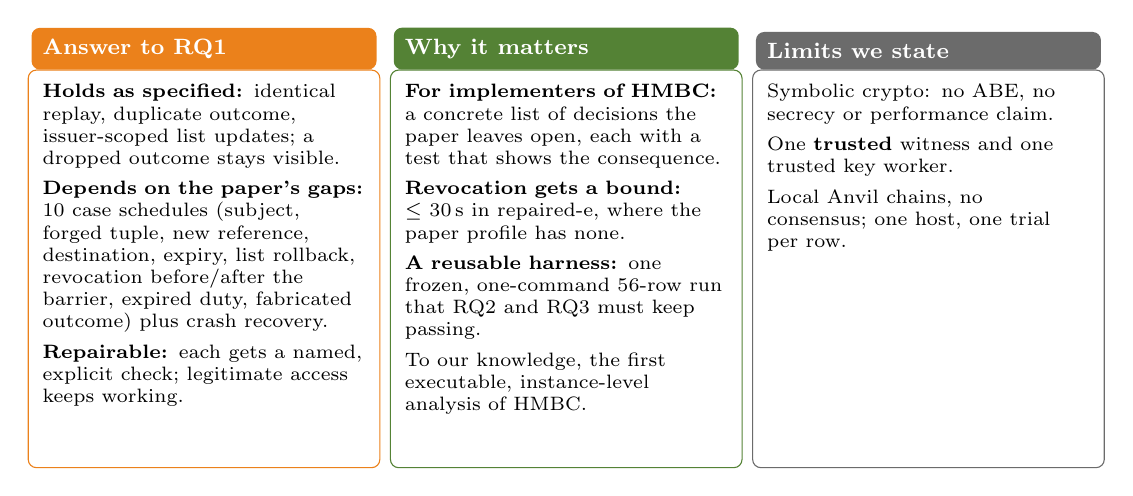
\begin{tikzpicture}[x=1cm, y=1cm, cw/.style={text width=4.1cm, draw=none, execute at begin node={\hyphenpenalty=10000\exhyphenpenalty=10000}}, hw/.style={text width=4.1cm, font=\footnotesize\bfseries}]
  \node[pcard=accent, cw] (k1) at (0,0) {%
    \textbf{Holds as specified:} identical replay, duplicate outcome, issuer-scoped list updates; a dropped outcome stays visible.\\[3pt]
    \textbf{Depends on the paper's gaps:} 10 case schedules (subject, forged tuple, new reference, destination, expiry, list rollback, revocation before/after the barrier, expired duty, fabricated outcome) plus crash recovery.\\[3pt]
    \textbf{Repairable:} each gets a named, explicit check; legitimate access keeps working.};
  \node[phead=accent, hw] at (0,0) {Answer to RQ1};
  \node[pcard=dbc, cw] (k2) at (4.6,0) {%
    \textbf{For implementers of HMBC:} a concrete list of decisions the paper leaves open, each with a test that shows the consequence.\\[3pt]
    \textbf{Revocation gets a bound:} $\le$ 30\,s in repaired-e, where the paper profile has none.\\[3pt]
    \textbf{A reusable harness:} one frozen, one-command 56-row run that RQ2 and RQ3 must keep passing.\\[3pt]
    To our knowledge, the first executable, instance-level analysis of HMBC.};
  \node[phead=dbc, hw] at (4.6,0) {Why it matters};
  \node[pcard=datagray, cw] (k3) at (9.2,0) {%
    Symbolic crypto: no ABE, no secrecy or performance claim.\\[3pt]
    One \textbf{trusted} witness and one trusted key worker.\\[3pt]
    Local Anvil chains, no consensus; one host, one trial per row.\\[3pt]};
  \node[phead=datagray, hw] at (9.2,0) {Limits we state};
  \foreach \k/\c in {1/accent, 2/dbc, 3/datagray} \draw[\c, rounded corners=3pt] (k\k.north west) rectangle ($(k\k.north east)+(0,-5.05)$);
\end{tikzpicture}

\vspace{0.5em}

\begin{tikzpicture}
  \node[draw=accent, fill=accent!10, rounded corners=3pt, text width=13.2cm, align=center, inner sep=5pt, font=\footnotesize]
    {Repaired-e puts all decision trust on \textbf{one witness}.\\RQ2 asks what survives when witnesses are Byzantine.};
\end{tikzpicture}
\note{The "first instance-level analysis" claim rests on our non-exhaustive literature search (slide 12). Repaired-e's pre-barrier case is accepted on purpose, inside the bounded window.}
\end{frame}

% ---------------------------------------------------------------- Next: F (and G)
\begin{frame}{Next: Phase RQ2, then RQ3}
\begin{columns}[T,onlytextwidth]
\column{0.60\textwidth}
\textbf{\textcolor{pbc}{RQ2: Byzantine operators}}\\[0.3em]
\centering
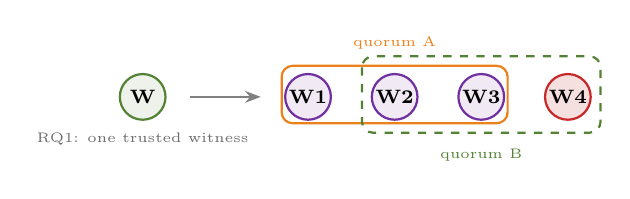
\begin{tikzpicture}[x=1cm, y=1cm, w/.style={circle, draw, thick, minimum size=0.58cm, font=\scriptsize\bfseries, inner sep=0pt}]
  \node[w, draw=dbc, fill=dbc!10] (e) at (0,0) {W};
  \node[font=\tiny, text=datagray, below=1pt of e] {RQ1: one trusted witness};
  \draw[->, thick, gray] (0.6,0) -- (1.5,0);
  \node[w, draw=pbc, fill=pbc!10] (w1) at (2.1,0) {W1};
  \node[w, draw=pbc, fill=pbc!10] (w2) at (3.2,0) {W2};
  \node[w, draw=pbc, fill=pbc!10] (w3) at (4.3,0) {W3};
  \node[w, draw=badred, fill=badred!15] (w4) at (5.4,0) {W4};
  \draw[accent, thick, rounded corners] ($(w1.north west)+(-0.12,0.18)$) rectangle ($(w3.south east)+(0.12,-0.12)$);
  \draw[dbc, thick, dashed, rounded corners] ($(w2.north west)+(-0.2,0.3)$) rectangle ($(w4.south east)+(0.2,-0.24)$);
  \node[font=\tiny, text=accent, anchor=south] at ($(w1.north)!0.5!(w3.north)+(0,0.18)$) {quorum A};
  \node[font=\tiny, text=dbc, anchor=north] at ($(w2.south)!0.5!(w4.south)+(0,-0.24)$) {quorum B};
\end{tikzpicture}\\[-0.05em]
{\tiny any two 3-of-4 quorums share $\ge$ 2 witnesses, so at least one honest one when $f=1$}

\raggedright\footnotesize
\begin{enumerate}\setlength{\itemsep}{1pt}
  \item \textbf{RQ2-01: freeze the fault model first:} $n=4$, $q=3$, $f=1$; a trust matrix over chains, relay, witnesses, CAs, key worker, client and store; expected results agreed before any run.
  \item \textbf{Ledger:} quorum verifier and governance certificates (distinct signers, set version, bound to action, nonce, expiry).
  \item \textbf{Protocol:} 4 independent witnesses; each stores its first signed decision, so it cannot equivocate.
  \item \textbf{Evaluation:} 0/1/2 faulty witnesses, equivocation, withholding, stale views, worker compromise; a TLA+/TLC model; RQ1's 56 rows re-run as regression.
\end{enumerate}

\column{0.37\textwidth}
\textbf{\textcolor{dbc}{RQ3: key lifecycle}}\\[0.3em]
\centering
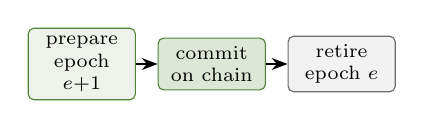
\begin{tikzpicture}[x=1cm, y=1cm, ep/.style={box, text width=1.15cm, minimum height=0.6cm}]
  \node[ep, draw=dbc, fill=dbc!10] (p) at (0,0) {prepare\\epoch $e{+}1$};
  \node[ep, draw=dbc, fill=dbc!20] (c) at (1.65,0) {commit\\on chain};
  \node[ep, draw=datagray, fill=gray!10] (r) at (3.3,0) {retire\\epoch $e$};
  \draw[->, thick] (p) -- (c);
  \draw[->, thick] (c) -- (r);
\end{tikzpicture}

\raggedright\footnotesize
\begin{itemize}\setlength{\itemsep}{1pt}
  \item Gate first: a real MA-CP-ABE adapter (Charm, Lewko–Waters) with a correct KSSC/user split.
  \item What stays secret after revocation, joining, a later key compromise, and for cached outputs.
  \item Measured encryption, decryption and rotation cost.
\end{itemize}
\end{columns}
\note{Board is at F0. F needs its own plan and the team's go-ahead before any F code; G stays locked until gate F passes (PLAN.md sections 6 and 7, GATES.md F and G checklists).}
\end{frame}

% ---------------------------------------------------------------- 18. Close
\begin{frame}[standout]
Thank you\\[0.5em]
{\normalsize Questions?}
\end{frame}

\end{document}
